\chapter{Range queries in the snapshot model}\label{section:range-snapshot}
\thispagestyle{myheadings}

	\acrfull{ope} and \acrfull{ore} are two important encryption schemes that have been proposed in the area of query evaluation over encrypted data.
	These schemes can provide very efficient query execution but at the same time may leak some information to adversaries.
	In this chapter, we present the first comprehensive comparison among a number of important \acrshort{ope} and \acrshort{ore} schemes using a framework that we developed.
	We evaluate protocols that are based on these schemes as well.
	We analyze and compare them both theoretically and experimentally and measure their performance over database indexing and query evaluation techniques using not only execution time but also \acrshort{io} performance and usage of cryptographic primitive operations.
	Our comparison reveals some interesting insights concerning the relative security and performance of these approaches in database settings.
	Furthermore, we propose a number of improvements for some of these scheme and protocols.
	Finally, we provide a number of suggestions and recommendations that can be valuable to database researchers and users.

	\emph{Some of the following sections were paraphrased or taken verbatim from the following published work.}

	\cite{ore-benchmark-17} \printpublication{ore-benchmark-17}

	\section{Introduction}

	Secure outsourced database systems aim at helping organizations outsource their data to untrusted third parties, without compromising data confidentiality or query efficiency.
	The main idea is to encrypt the data records before uploading them to an untrusted server along with an index data structure that governs which encrypted records to retrieve for each query.
	While strong cryptographic tools can be used for this task, existing implementations such as CryptDB \cite{crypt-db}, Cipherbase \cite{cipherbase-daas}, StealthDB \cite{stealth-db} and TrustedDB \cite{trusted-db} try to optimize performance but do not provide strong security guarantees when answering queries.
	Indeed, a series of works \cite{multidimensional-range-queries, inference-attack-islam-14, leakage-abuse-attacks-cash-15, inference-attacks-naveed-15, generic-attacks-kellaris, attacks-tao-of-inference, grubbs-attacks, access-pattern-disclosure, attacks-improved-reconstruction} demonstrate that these systems are vulnerable to a variety of reconstruction attacks.
	That is, an adversary can fully reconstruct the distribution of the records over the domain of the indexed attribute.
	This weakness is prominently due to the \emph{access pattern leakage}: the adversary can tell if the same encrypted record is returned on different queries.

	More recently, \cite{generic-attacks-kellaris, state-of-uniform, attacks-improved-reconstruction, pump-volume-attacks, volume-range-attacks} showed that reconstruction attacks are possible even if the systems employ heavyweight cryptographic techniques that hide the access patterns, such as homomorphic encryption \cite{arbitrary-functions-encrypted, fully-homomorphic-encryption} or \acrfull{oram} \cite{oram-theory, oram-original}, because they leak the size of the result set of a query to the server (this is referred to as \emph{communication volume leakage}). % chktex 2
	Thus, even some recent systems that provide stronger security guarantees like ObliDB \cite{oblidb}, Opaque \cite{opaque} and Oblix \cite{oblix} are susceptible to these attacks. % chktex 2
	This also means that no outsourced database system can be both optimally efficient and privacy-preserving: secure outsourced database systems should not return the exact number of records required to answer a query.

	We take the next step towards designing secure outsourced database systems by presenting novel constructions that strike a provable balance between efficiency and privacy.
	First, to combat the access pattern leakage, we integrate a layer of \acrshort{oram} storage in our construction.
	Then, we bound the communication volume leakage by utilizing the notion of \acrfull{dp} \cite{differential-privacy-original}.
	Specifically, instead of returning the exact number of records per query, we only reveal perturbed query answer sizes by adding random encrypted records to the result so that the communication volume leakage is bounded.
	Our construction guarantees privacy of any single record in the database which is necessary in datasets with stringent privacy requirements.
	In a medical \acrshort{hipaa}-compliant setting, for example, disclosing that a patient exists in a database with a rare diagnosis correlating with age may be enough to reveal a particular individual.

	The resulting mechanism achieves the required level of privacy, but implemented na\"{\i}vely the construction is prohibitively slow.
	We make the solution practical by limiting the amount of noise and the number of network roundtrips while preserving the privacy guarantees.
	We go further and present a way to parallelize the construction, which requires adapting noise-generation algorithms to maintain differential privacy requirements.

	Using our system, we have run an extensive set of experiments over cloud machines, utilizing large datasets --- that range up to 10 million records --- and queries of different sizes, and we report our experimental results on efficiency and scalability.
	We compare against best possible solutions in terms of efficiency (conventional non-secure outsourced database systems on unencrypted data) and against an approach that provides optimal security (retrieves the full table from the cloud or runs the entire query obliviously with maximal padding).
	We report that our solution is very competitive against both baselines.
	Our performance is comparable to that of unsecured plain-text optimized database systems (like MySQL and PostgreSQL): while providing strong security and privacy guarantees, we are only 4 to 8 times slower in a typical setting.
	Compared with the optimally secure solution, a linear scan (downloading all the records), we are 18 times faster in a typical setting and even faster as database sizes scale up.

	\smallskip

	To summarize, our contributions in this work are as follows:
	\begin{itemize}
		\item
			We present a new model for a \emph{differentially private} outsourced database system, \acrshort{cdpodb}, its security definition, query types, and efficiency measures.
			In our model, the adversarial honest-but-curious server cannot see the record values, access patterns, or exact communication volume.

		\item
			We describe a novel construction, \epsolute{}, that satisfies the proposed security definition, and provide detailed algorithms for both range and point query types.
			In particular, to conceal the access pattern and communication volume leakages, we provide a secure storage construction, utilizing a combination of \acrlong{oram} \cite{oram-theory, oram-original} and differentially private sanitization \cite{non-interactive-database-privacy}.
			Towards this, we maintain an index structure to know how many and which objects we need to retrieve.
			This index can be stored locally for better efficiency (in all our experiments this is the case), but crucially, it can also be outsourced to the adversarial server and retrieved on-the-fly for each query.

		\item
			We improve our generic construction to enable parallelization within a query.
			The core idea is to split the storage among multiple \acrshortpl{oram}, but this requires tailoring the overhead required for differential privacy proportionally to the number of \acrshortpl{oram}, in order to ensure privacy.
			We present practical improvements and optimization techniques that dramatically reduce the amount of fetched noise and the number of network roundtrips.

		\item
			Finally, we provide and open-source a high-quality C++ implementation of our system.
			We have run an extensive set of experiments on both synthetic and real datasets to empirically assess the efficiency of our construction and the impact of our improvements.
			We compare our solutions to the na\"{\i}ve approach (linear scan downloading all data every query), oblivious processing and maximal padding solution (Shrinkwrap \cite{shrinkwrap}), and to a non-secure regular \acrshort{rdbms} (PostgreSQL and MySQL), and we show that our system is very competitive.
	\end{itemize}

	\subsection{Related Work}

		We group the related secure databases, engines, and indices into three categories
		\begin{enumerate*}[label={(\roman*)}]
			\item systems that are oblivious or volume-hiding and do not require \acrfull{tee},
			\item constructions that rely on \acrshort{tee} (usually, Intel \acrshort{sgx}),
			\item solutions that use property-preserving or semantically secure encryption and target primarily a snapshot adversary.
		\end{enumerate*}
		\emph{We claim that \epsolute{} is the most secure and practical range- and point-query engine in the outsourced database model, that protects both \acrfull{ap} and \acrfull{cv} using \acrlong{dp}, while not relying on \acrshort{tee}, linear scan or padding result size to the maximum.}

		\paragraph*{Obliviousness and volume-hiding without enclave}

			This category is the most relevant to \epsolute{}, wherein the systems provide either or both \acrshort{ap} and \acrshort{cv} protection without relying on \acrshort{tee}.
			\crypte{} \cite{crypte} is a recent end-to-end system executing ``\acrshort{dp} programs''.
			\crypte{} has a different model than \epsolute{} in that it assumes two non-colluding servers, an adversarial querying user (the analyst), and it uses \acrshort{dp} to protect the privacy of an individual in the database, which includes volume-hiding for aggregate queries.
			\crypte{} also does not consider oblivious execution and attacks against the \acrshort{ap}.
			Shrinkwrap \cite{shrinkwrap} (and its predecessor SMCQL \cite{smcql}) is an excellent system designed for complex queries over federated and distributed data sources.
			In Shrinkwrap, \acrshort{ap} protection is achieved by using oblivious operators (linear scan and sort) and \acrshort{cv} is concealed by adding fake records to intermediate results with \acrshort{dp}.
			Padding the result to the maximum size first and doing a linear scan over it afterwards to ``shrink'' it using \acrshort{dp}, is much more expensive than in \epsolute{}, however.
			In addition, in processing a query, the worker nodes are performing an $O(n \log{n})$ cost oblivious sorting, where $n$ is the maximum result size (whole table for range query), since they are designed to answer more general complex queries.
			SEAL \cite{seal} offers adjustable \acrshort{ap} and \acrshort{cv} leakages, up to specific bits of leakage.
			SEAL builds on top of Logarithmic-SRC \cite{practical-range-search}, splits storage into multiple \acrshortpl{oram} to adjust \acrshort{ap}, and pads results size to a power of 2 to adjust \acrshort{cv}.
			\epsolute{}, on the other hand, fully hides the \acrshort{ap} and uses \acrshort{dp} with its guarantees to pad the result size.
			PINED-RQ \cite{pined-rq} samples Laplacian noise right in the B+ tree index tree, adding fake and removing real pointers according to the sample.
			Unlike \epsolute{}, PINED-RQ allows false negatives (i.e., result records not included in the answer), and does not protect against \acrshort{ap} leakage.
			On the theoretical side, \textcite{differential-obliviousness} (followed by \textcite{differential-obliviousness-followup}) treat the \acrshort{ap} itself as something to protect with \acrshort{dp}.
			\cite{differential-obliviousness} introduces a notion of differential obliviousness that is admittedly weaker than the full obliviousness used in \epsolute{}. % chktex 2
			Most importantly, \cite{differential-obliviousness} ensures differential privacy w.r.t.~the \acrshort{oram} only, while \epsolute{} ensures \acrshort{dp} w.r.t.~the entire view of the adversary. % chktex 2

		\paragraph*{Enclave-based solutions}

			Works in this category use trusted execution environment (usually, \acrshort{sgx} enclave).
			These works are primarily concerned with the \acrshort{ap} protection for both trusted and untrusted memory, unlike \epsolute{} which also protects \acrshort{cv}.
			Cipherbase \cite{cipherbase-daas} was a pioneer introducing the idea of using \acrshort{tee} (\acrshort{fpga} at that time) to assist with \acrshort{rdbms} security.
			HardIDX \cite{hardidx} simply puts the B+ tree in the enclave, while StealthDB \cite{stealth-db} symmetrically encrypts all records and brings them in the enclave one at a time for processing.
			EnclaveDB \cite{enclave-db} assumes somewhat unrealistic \SI{192}{\giga\byte} enclave and puts the entire database in it.
			ObliDB \cite{oblidb} and Opaque \cite{opaque} assume fully oblivious enclave memory (not available as of today) and devise algorithms that use this fully trusted portion to obliviously execute common \acrshort{rdbms} operators, like filters and joins.
			Oblix \cite{oblix} provides a multimap that is oblivious both in and out of the enclave.
			HybrIDX claims protection against both \acrshort{ap} and \acrshort{cv} leakages, but unlike \epsolute{} it only obfuscates them.
			\epsolute{} offers an indistinguishability guarantee for \acrshort{ap} and a \acrshort{dp} guarantee for \acrshort{cv}, while HybrIDX hides the exact result size and only obfuscates the \acrshort{ap}.
			Lastly, Hermetic \cite{hermetic} takes on the \acrshort{sgx} side-channel attacks, including \acrshort{ap}.
			It provides oblivious primitives, however, it only offers protection against software and not physical attacks (e.g., it trusts a hypervisor to disable interrupts).

		\paragraph*{Solutions against the snapshot adversary}

			Works in this category protect against the snapshot adversary, which takes a snapshot of the data at a fixed point in time (e.g., stolen hard drive).
			We stress that \epsolute{} provides semantic security against the snapshot adversary on top of \acrshort{ap} and \acrshort{cv} protection.
			CryptDB \cite{crypt-db} is a seminal work in this direction offering computations over encrypted data.
			It has since been shown (e.g. \cite{inference-attacks-naveed-15,inference-attack-islam-14,attacks-tao-of-inference}) that the underlying property-preserving schemes allow for reconstruction attacks.
			Arx \cite{arx} provides strictly stronger security guarantees by using only semantically secure primitives.
			Seabed \cite{seabed} uses an additively symmetric homomorphic encryption scheme for aggregates and certain filter queries.
			\textcite{ppqed} offer a method to verify and apply a predicate (a junction of conditions) using garbled circuits or homomorphic encryption without revealing the predicate itself.
			SisoSPIR \cite{sisospir} presents a mechanism to build an oblivious index tree such that neither party learns the pass taken.
			See \cite{ore-benchmark-17} for a survey of range query protocols in this category. % chktex 2


	\section{Security Perspective}\label{section:range-snapshot:security}

	Each scheme and protocol we analyze has its own security definition, which captures different leakage levels.
	We attempt to unify these definitions and analyze them under a common framework.
	We also attempt to assess relative security of these definitions and analyze their leakages.

	In this work we mostly consider the snapshot model, where the attacker can observe all the database contents at one time instant.
	Note that this excludes timing attacks such as measuring encryption time.
	All security definitions of the schemes and protocols that we discuss here are based on this model.
	Also, the snapshot attacker is the most common attacker that we face today \cite{secure-queries-overview}.
	The idea is that a hacker or an insider can steal the entire encrypted database and all its contents at some point in time.

	Beyond the snapshot model, it is also possible to consider a stronger adversary who can track communication volume and data access patterns in real time.
	Approaches that help protect against such an attacker include ORAM for protection against access pattern leakage and differential privacy for protection against communication volume leakage.
	Although this model is not a primary target of this paper, our benchmark includes a protocol (\cref{section:range-snapshot:oram}) that is secure in this setting to show the cost of adding such protection.

	We wanted to specifically comment on a work of \textcite{leakage-abuse-grubs-2017}, which demonstrates a series of attacks against OPE and ORE schemes.
	The attacks can be very successful, but they depend on certain prerequisites.
	First, all attacks assume the existence of a well-correlated auxiliary dataset.
	Second, the binomial attack, which works against a ``perfectly secure frequency-hiding scheme'', reliably recovers only high-frequency elements.
	Finally, the attacks are specifically devastating against encrypted strings (e.g.\ first and last names) as opposed to numerical data, and we also do not recommend using OPE / ORE for strings (see \cref{section:range-snapshot:variable-inputs}).
	One of the conclusions of our work is that security is negatively correlated with performance and it is up to a practitioner to trade off security and performance constraints.

	\subsection{A note on variable-length inputs}\label{section:range-snapshot:variable-inputs}

		A generic OPE / ORE scheme accepts bit-strings of any length as inputs, and treats them as numbers or processes them bit-by-bit.
		We warn against supplying raw bytes of variable length (e.g.\ encoded strings) to OPE and ORE schemes, as such an approach will introduce both performance and security challenges.

		From the performance standpoint, the complexity of OPE / ORE schemes usually depends on the input length at least linearly (see \cref{table:primitive-usage-theory}).
		32-bit numbers already introduce a noticeable overhead for some (usually more secure) schemes, and supplying arbitrary-length inputs may worsen performance by at least an order of magnitude.

		Security of such a construction will be minimal as most schemes leak some information about the magnitude of the difference, and longer inputs will naturally be treated as larger numbers.
		Thus, the difference between long and short inputs will be apparent.
		We refer to the work of~\textcite{leakage-abuse-grubs-2017} as they have a practically supported discussion of security consequences of using OPE / ORE with arbitrary strings.

		On the other hand, other protocols in our benchmark can usually handle variable-length inputs as long as they fit into a single block for the underlying block cipher.


	\section{OPE and ORE Schemes}

	An Order-Revealing Encryption scheme is a triple of polynomial\hyp{}time algorithms $\setup$, $\encrypt$ and $\compare$.
	$\setup$ generates a key of parameterized length (the $\lambda$ parameter).
	$\encrypt$ takes a numerical input (as a bit string) and produces a ciphertext.
	$\compare$ takes two ciphertexts generated by the scheme and outputs whether the first plaintext was strictly less than the second.
	Note that being able to check this condition is enough to apply all other comparison operators ($<$, $\le$, $=$, $\ge$, $>$).
	Also note that an ORE scheme does not include a decryption algorithm, because one can simply append a symmetric encryption of the plaintext to the produced ciphertext and use it for decryption.\footnote{
		\emph{Given the secret key}, it is possible to decrypt a ciphertext by doing binary search on the plaintext domain: encrypting known values and comparing them against the target ciphertext, until the target plaintext is found.
		However, this would require $\bigO{\log{|\domain|}}$ encryption and comparison operations.
	}
	An Order-Preserving Encryption (OPE) scheme is a particular case of an ORE scheme where ciphertexts are numerical and thus $\compare$ routine is trivial (the numerical order of ciphertexts is the same as underlying plaintexts).
	OPE may optionally include a decryption algorithm, since appending a symmetric ciphertext is no longer possible.

	Both OPE and ORE schemes by definition allow to totally order the ciphertexts.
	This is their inherent leakage (by design) and all the OPE / ORE security definitions account for this and possibly additional leakage.

	We proceed by describing and analyzing the OPE / ORE schemes we have benchmarked.
	All plaintexts are assumed to be 32-bit signed integers, or $n$-bit inputs in complexity analysis.
	OPE ciphertexts are assumed to be 64-bit signed integers.

	From here, we will use the term ORE to refer to both OPE and ORE, unless explicitly stated otherwise.
	Each scheme has its own subsection where the first part is the construction overview followed by security discussion, and the second part is our theoretical and experimental analysis.

	% cSpell:ignore Lewi BCLO CLWW captionsetup

\begin{sidewaystable}
	\renewcommand{\arraystretch}{1.5}
	\centering
	\captionsetup{width=\textwidth}
	\caption[Primitive usage by \acrshort{ope} / \acrshort{ore} schemes]{
		\cite[Tables 1 and 4]{ore-benchmark-17}.
		Primitive usage by \acrshort{ope} / \acrshort{ore} schemes.
		Ordered by security rank --- most secure below.
		$n$ is the input length in bits, $d$ is a block size for Lewi-Wu~\cite{lewi-wu-ore} scheme, $\lambda$ is a \acrshort{prf} output size, $N$ is a total data size, \textbf{\acrshort{hg}} is a hyper-geometric distribution sampler, \textbf{\acrshort{pph}} is a property-preserving hash with $h$-bit outputs built with bilinear maps and \textbf{bolded} are weak points of the schemes.
		Values in parentheses are simulation-derived. $N = 10^3$, $n = 32$, $d = 2$, $\lambda = 128$ and $h = 128$ in this simulation.
	}\label{tbl:primitive-usage-theory}
	\begin{tabular*}{\linewidth}{ !{\extracolsep\fill} l c c c c c } % chktex 26

		\toprule

		\multirow{2}{*}{Scheme}						& \multicolumn{2}{c}{Primitive usage (number of invocations)}																				& \multirow{2}{*}{\makecell{Ciphertext size, \\ or state size (bits)}}					&  \multirow{2}{*}{\makecell{Leakage \\ (in addition to inherent total order)}}				\\ \cline{2-3}
		\rule{0pt}{10pt}							& Encryption																& Comparison													& 																						& 																							\\

		\toprule

		\cite{bclo-ope}								& $\bm{\approx n}$ \textbf{(41) \acrshort{hg}}								& none															& $2n$ (64)																				& \textbf{$\approx$ Top half of the bits}													\\

		\midrule

		\cite{clww-ore}								& $n$ (32) \acrshort{prf} 													& none															& $2n$ (64)																				& \textbf{Most-significant differing bit}													\\

		\midrule

		\multirow{3}{*}{\cite{lewi-wu-ore}}			& \boldmath{} $\nicefrac{2n}{d}$ \unboldmath{} \textbf{(32) \acrshort{prp}}	& \multirow{3}{*}{$\frac{n}{2d}$ (9) Hash}						& 																						& \multirow{3}{*}{Most-significant differing block}											\\
													& $2 \frac{n}{d} \left( 2^d + 1 \right)$ (160) \acrshort{prf}				&																& $\frac{n}{d} \left(\lambda + n + 2^{d + 1} \right) + \lambda$							&																							\\
													& $\frac{n}{d} 2^d$ (64) Hash												&																& (2816)																				&																							\\


		\midrule

		\multirow{3}{*}{\cite{parameter-hiding-ore}}			& $n$ (32) \acrshort{prf}													& \multirow{3}{*}{$\bm{n^2}$ \textbf{(1046) \acrshort{pph}}}	& \multirow{3}{*}{$n \cdot h$ (4096)}													& \multirow{3}{*}{\makecell{Equality pattern \\ of the most-significant \\ differing bit}}	\\
													& $n$ (32) \acrshort{pph}													&																&																						& 																							\\
													& 1 \acrshort{prp}															&																&																						& 																							\\

		\midrule

		\cite{fh-ope}								& 1 Traversal																& 3 Traversals													& $\bm{3 \cdot n \cdot N}$ \textbf{(86842)}												& Insertion order																			\\

		\bottomrule

	\end{tabular*}
\end{sidewaystable}


	\subsection{BCLO OPE}

	The OPE scheme by \textcite{bclo-ope} was the first OPE scheme that provided formal security guarantees and was used in one of the first database systems that executes queries over encrypted data (CryptDB \cite{crypt-db}).
 	The core principle of their construction is the natural connection between a random order-preserving function and the hypergeometric probability distribution.

	The encryption algorithm works by splitting the domain into two parts according to a value sampled from the hypergeometric distribution ($\hg$) routine, and splitting the range in half recursively.
	When the domain size contains a single element, the corresponding ciphertext is sampled uniformly from the current range.

	All pseudo-random decisions are made by an internal PRG ($\tapegen$ in \cite{bclo-ope}).
	This way not only the algorithm is deterministic, but also decryption is possible.
	The decryption procedure takes the same ``path'' of splitting domain and range, and when the domain size reaches one, the only value left is the original plaintext.

	\subsubsection{Security}
		This scheme is POPF-CCA secure \cite{bclo-ope}, meaning that it is as secure as the underlying ideal object --- randomly sampled order-preserving function from a certain domain to a certain range.
		For practical values of the parameters, \textcite{ope-leakage} showed that the distance between the plaintexts can be approximated to an accuracy of about the square root of the domain size.
		In other words, approximately, half of the bits (the most significant) are leaked.
		\textcite{leakage-abuse-grubs-2017} showed that this leakage allows to almost entirely decrypt the ciphertexts (given auxiliary data with a similar distribution) and encrypting strings (rather than numbers) with this scheme is especially dangerous (see \cref{section:range-snapshot:variable-inputs}).

	\subsubsection{Analysis and implementation challenges}

		Efficient sampling from the hypergeometric distribution is a challenge by itself.
		Authors suggest using a randomized yet exact (not approximate) Fortran algorithm by \textcite{hg-sampler}.
		It should be noted that the algorithm relies on infinite precision floating-point numbers, which most regular frameworks do not have.
		The security consequences of finite precision computations is actually an open question.
		The complexity of this randomized algorithm is hard to analyze; however, we empirically verified that its running time is no worse than linear in the input bit length.
		The authors also suggest a different algorithm for smaller inputs \cite{hg-sampler-small}.

		On average, encryption and decryption algorithms make $n$ calls to $\hg$, which in turn consumes entropy generated by the internal PRG\@.
		The entropy, and thus the number of calls to PRG, needed for one $\hg$ run is hard to analyze theoretically.
		However, we derived this number experimentally (see \cref{section:range-snapshot:evaluation}).

		BCLO has been implemented in numerous languages and has been deployed in a number of secure systems.
		We add {\Csharp} implementation to the list, and recommend using a library that supports infinite precision floating-point numbers when building the hypergeometric sampler.

	\subsection{CLWW \texorpdfstring{\acrshort{ore}}{ORE} \texorpdfstring{\cite{clww-ore}}{}}\label{section:range-snapshot:clww}

	The \acrshort{ore} scheme by \textcite{clww-ore}, which authors call ``Practical ORE'', is the first efficient \acrshort{ore} implementation based on \acrshortpl{prf}.

	On encryption, the plaintext is split into $n$ values in the following way.
	For each bit, a value is this bit concatenated with all more significant bits.
	This value is given to a keyed \acrshort{prf} and the result is numerically added to the next less significant bit.
	This resulting list of $n$ elements is the ciphertext.

	The comparison routine traverses two lists in-order looking for the case when one value is greater than the other by exactly one, revealing location and value of the first differing bit.
	If no such index exists, the plaintexts are equal.

	\subsubsection{Security}

		A generic \acrshort{ore} security definition was introduced along with the scheme \cite{clww-ore}.
		\acrshort{ore} leakage is more clearly quantified than in \acrshort{ope}.
		The definition says that the scheme is secure with a leakage $\leak(\cdot)$ if there exists an algorithm (simulator) that has access to the leakage function and can generate output indistinguishable from the one generated by the real scheme.
		This scheme satisfies \acrshort{ore} security definition with the leakage $\leak(\cdot)$ of the location and value of the first differing bit of every pair of plaintexts.
		Note that the most significant differing bit also leaks the approximate distance between two values.

	\subsubsection{Analysis and implementation challenges}

		On encryption the algorithm makes $n$ calls to \acrshort{prf} and the comparison procedure does not use any cryptographic primitives.
		Ciphertext is a list of length $n$, where each element is an output of a \acrshort{prf} modulo 3.
		The authors claim that the ciphertext's size is $n \log_2 3$, just $1.6$ times larger than the plaintext's size.
		While this may be true for large enough $n$ if ternary encoding is used, we found that in practice the ciphertext size is still $2n$.
		$1.6 n$ for 32-bit words is $51.2$ bits, which will have to occupy one 64-bit word, or two 32-bit words, therefore resulting in $2n$ anyway.

	\subsection{Lewi-Wu \acrshort{ore}}

	\textcite{lewi-wu-ore} presented an improved version of the CLWW scheme \cite{clww-ore} which leaks strictly less.

	The novel idea was to use the ``left / right framework'' in which two ciphertexts get generated --- left and right.
	The right ciphertexts are semantically secure, so an adversary will learn nothing from them.
	Comparison is only defined between the left ciphertext of one plaintext and the right ciphertext of another plaintext.

	The approach is to split the plaintext into blocks of $d$ bits.
	The ciphertext is computed block-wise.
	For the right side, the algorithm compares the given block value to all $2^d$ possible block values; each comparison result is added (modulo 3) to a \acrshort{prf} of the previous blocks.
	All $2^d$ comparison results go into the right ciphertext.
	The left side, which is shorter, is produced in such a way as to reveal the correct comparison result.
	This way the location of the differing bit inside the block is hidden, but the location of the first differing block is revealed.

	\subsubsection{Security}
		This scheme satisfies the \acrshort{ore} security definition introduced by~\textcite{clww-ore} with the leakage $\leak(\cdot)$ of the location of the first differing \emph{block}.
		This property allows a practitioner to set performance-security tradeoff by tuning the block size.
		Left / right framework is particularly useful in a {\BPlus} tree since it is possible to store only one (semantically secure) side of a ciphertext in the structure (see \cref{section:range-snapshot:ore-to-protocol}).

	\subsubsection{Analysis and implementation challenges}

		Let $n$ be the size of input in bits (e.g.\ 32) and $d$ be the number of bits per block (e.g.\ 2).

		Left encryption loops $\frac{n}{d}$ times making one \acrshort{prp} call and two \acrshort{prf} calls each iteration.
		Right encryption loops $\frac{n}{d} 2^d$ times making one \acrshort{prp} call, one hash call and two \acrshort{prf} calls each iteration.
		Comparison makes $\frac{n}{d}$ calls to hash at worst and half of that number on average.
		Please note that the complexity of right encryption is exponential in the block size.
		In the \cref{table:primitive-usage-theory} the \acrshort{prp} usage is linear due to our improvement.
		The ciphertext size is no longer negligible --- $\frac{n}{d} \left(\lambda + n + 2^{d + 1} \right) + \lambda$, for $\lambda$ being \acrshort{prf} output size.

		The implementation details of this approach raise an interesting security question.
		Although the authors suggest using 3-rounds Feistel networks \cite{unbalanced-feistel} for \acrshort{prp} and use it in their implementation, it may not be secure for small input sizes.
		Feistel networks security depends on the input size \cite{feistel-security} --- exponential in the input size.
		However, the typical input for \acrshort{prp} in their scheme is 2--8 bits, thus even exponential number is small.

		We have considered multiple \acrshort{prp} implementations to use instead of the Feistel networks.
		Because the domain size is small (from $2^2$ to $2^8$ elements), we have decided to build a \acrshort{prp} by simply using the key as an index into the space of all possible permutations on the domain, where a permutation is obtained from the key via Knuth shuffle (this approach was mentioned in \cite{knuth-shuffle-security}).
		Another important aspect of the implementation is that for each block we need to compute the permutation of all the values inside the block.
		This operation applied many times can be expensive.
		To address this, we propose to generate a \acrshort{prp} table once for the whole block and then use this table when one needs to compute the location of an element of permutation.
		This can reduce the \acrshort{prp} usage (indeed, we observe a reduction from 80 to 32 calls in our case).
		We evaluate this improved approach in our experimental section.


	% cSpell:ignore Kerschbaum captionsetup

\begin{sidewaystable}
	\renewcommand{\arraystretch}{1.5}
	\centering
	\captionsetup{width=\textwidth}
	\caption[Performance of the range query protocols]{
		\cite[Tables 2 and 3]{ore-benchmark-17}.
		Performance of the range query protocols.
		Ordered by security rank --- most secure below.
		$N$ is a total data size, $B$ is an \acrshort{io} page size, $L$ is a POPE tree branching factor, $r$ is the result size in records and \textbf{bolded} are weak points of the protocols.
		The cell content is structured as follows: top value is the analytical result in $\mathcal{O}$ notation, bottom value is the number of requests for \acrshort{io} requests or number of messages and their total size for communication.
		In these experiments, $N = 247K$, $B = \SI{4}{\kilo\byte}$, $r \approx 247K \cdot \SI{0.5}{\percent} = 1235$, and $L = 60$.
	}\label{table:protocols}
	\begin{tabular*}{\linewidth}{ !{\extracolsep\fill} c c c c c c } % chktex 26

		\toprule

		\multirow{2}{*}{Protocol}			& \multicolumn{2}{c}{\acrshort{io} requests}																																			& \multirow{2}{*}{Leakage}						& \multicolumn{2}{c}{Communication}																																										\\ \cline{2-3} \cline{5-6}
		\rule{0pt}{10pt}					& Construction														& Query																												&												& Construction																						& Query 																							\\

		\toprule

		\makecell{{\BPlus} tree \\ with \acrshort{ore}}	& \makecell{$\log_B \frac{N}{B}$ \\ 3 requests}						& \makecell{$\log_B \frac{N}{B} + \frac{r}{B}$ \\ 44 requests}														& \textbf{Same as \acrshort{ore}}				& \makecell{$1$ \\ 2 / \SI{177}{\byte}}																& \makecell{$1$ \\ 2 / \SI{342}{\byte}}																\\

		\midrule

		\cite{florian-protocol}				& \makecell{$\bm{\frac{N}{B}}$ \\ \textbf{494 requests}}			& \makecell{$\log_2 \frac{N}{B} + \frac{r}{B}$ \\ 17 requests}														& \textbf{Total order}							& \makecell{$\log_2 N$ \\ 40 / \SI{671}{\byte}}														& \makecell{$\log_2 N$ \\ 86 / \SI{1453}{\byte}}													\\

		\midrule

		\makecell{\cite{pope} \\ warm}					& \multirow{2}{*}{\makecell{$1$ \\ 1 request}}						& \makecell{$\log_L \frac{N}{B} + \frac{r}{B}$ \\ 300 requests}														& \textbf{Partial order}						& \multirow{2}{*}{\makecell{$1$ \\ 2 / \SI{32}{\byte}}}												& \makecell{$\log_L N$ \\ 914 / \SI{347}{\kilo\byte}}												\\ \cline{1-1} \cline{3-3} \cline{6-6}

		\makecell{\cite{pope} \\ cold}					& 																	& \makecell{$\bm{{\nicefrac{N}{B}}}$ \\ \textbf{2175 requests}}														& Fully hiding									& 																									& \makecell{$\bm{N}$ \\ \textbf{498K / \SI[detect-all=true]{9}{\mega\byte}}}						\\

		\midrule

		\cite{practical-range-search}		& \textbf{---}														& \makecell{$\bm{r}$ \\ \textbf{40 requests}}																		& Same as \acrshort{sse}						& \textbf{---}																						& \makecell{$\log_2 N$ \\ 2 / \SI{391}{\byte}}														\\

		\midrule

		\acrshort{oram}						& \makecell{$\bm{{ \log^2 \frac{N}{B} }}$ \\ \textbf{31 requests}}	& \makecell{$\bm{{ \log_2 \frac{N}{B} \left( \log_B \frac{N}{B} + \frac{r}{B} \right) }}$ \\ \textbf{185 requests}}	& \makecell{Fully hiding \\ (access pattern)}	& \makecell{$\bm{{ \log^2 \frac{N}{B} }}$ \\ \textbf{143 / \SI[detect-all=true]{18}{\kilo\byte}}}	& \makecell{$\bm{{ \log^2 \frac{N}{B} }}$ \\ \textbf{490 / \SI[detect-all=true]{63}{\kilo\byte} }}	\\

		\bottomrule

	\end{tabular*}
\end{sidewaystable}


	\subsection{CLOZ \texorpdfstring{\acrshort{ore}}{ORE}}

	\textcite{parameter-hiding-ore} introduced a new \acrshort{ore} scheme that provably leaks less than any previous scheme.
	The idea is to use \textcite{clww-ore} construction (see \cref{section:range-snapshot:clww}), but permute the list of \acrshort{prf} outputs.
	The original order of those outputs is not necessary, as one can simply find a pair that differs by one.
	This is not enough to reduce leakage, however, since an adversary can count how many elements two ciphertexts have in common.

	To address this problem, the authors define a new primitive they call a \acrfull{pph}.
	A \acrshort{pph} as defined and used in \cite{parameter-hiding-ore}, allows one to expose a property (specifically $y \overset{?}{=} x + 1$) of two (numerical) elements such that nothing else is leaked.
	In particular, the outputs are randomized, so same element hashed twice will have different hashes.
	Please refer to the original paper \cite{parameter-hiding-ore} for formal correctness and security definitions.

	Equipped with the \acrshort{pph} primitive, the algorithm ``hashes'' the elements of the ciphertexts before outputting them.
	Due to security of \acrshort{pph}, the adversary would not be able to count how many elements two ciphertexts have in common, thus, would not be able to tell the location of differing bit.

	\subsubsection{Security}

		The strong side of the scheme is its security.
		The scheme leaks $\leak(\cdot)$ an \emph{equality pattern} of the most-significant differing bits (satisfying \textcite{clww-ore} definition).
		As defined in \cite{parameter-hiding-ore}, the intuition behind equality pattern is that for any triple of plaintexts $m_1$, $m_2$, $m_3$, it leaks whether $m_2$ differs from $m_1$ before $m_3$ does. % chktex 2
		We do not know of any attacks against this construction (partially because no implementation exists yet, see next subsection), but it is inherently vulnerable to frequency attacks that apply to all frequency-revealing \acrshort{ore} schemes (see \cref{section:range-snapshot:security}).

	\subsubsection{Analysis and implementation challenges}

		On encryption, the scheme makes $n$ calls to \acrshort{prf}, $n$ calls to \acrshort{pph} \algo{Hash} and one call to \acrshort{prp}.
		Comparison is more expensive, as the scheme makes $n^2$ calls to \acrshort{pph} \algo{Test}.

		The scheme has two limitations that make it impractical.
		The first one is the square number of calls to \acrshort{pph}, which is around $1024$ for a single comparison.

		The second problem is the \acrshort{pph} itself.
		Authors suggest a construction based on bilinear maps.
		The hash of an argument is an element of a group, and the test algorithm is computing a pairing.
		This operation is very expensive --- order of magnitude more expensive than any other primitive we have implemented for other schemes.

		We have implemented this scheme in C++ using the PBC library \cite{pbc} to empirically assess schemes's performance, and on our machine (see \cref{section:range-snapshot:evaluation}), a single comparison takes 1.9 seconds on average.
		Although we have produced the first (correct and secure) real implementation of this scheme in C++, it is infeasible to use it in the benchmark (it will take years to complete a single run).
		Therefore, for the purposes of our benchmark, we implemented a ``fake'' version of \acrshort{pph} --- correct, but insecure, which does not use pairings.
		Consequently, in our analysis we did not benchmark the speed of the scheme, but measured all other data.

	\subsection{FH-OPE}

	Frequency-hiding OPE by \textcite{fh-ope} is a stateful scheme that hides the frequency of the plaintexts, so the adversary is unable to construct a frequency histogram.

	This scheme is stateful, which means that the client needs to keep a data structure and update it with every encryption and decryption.
	The data structure is a binary search tree where the node's value is the plaintext and node's position in a tree is the ciphertext.
	For example, consider the range $[1, 128]$.
	Any plaintext that happens to arrive first (for example, $6$), will be the root, and thus the ciphertext is $64$.
	Then any plaintext smaller than the root, say $3$, will become the left child of the root, and will produce the ciphertext $32$.
	To encrypt a value, the algorithm traverses the tree until it finds a spot for the new plaintext, or finds the same plaintext.
	If the same plaintext is found, the traversal pseudo-randomly passes to the left or right child, up to the leaf.
	This way, the invariant of the tree --- intervals of the same plaintexts do not overlap --- is maintained.
	The ciphertext generated from the new node's position is returned.

	Due to randomized ciphertexts, the comparison algorithm is more complicated than in the regular deterministic OPE\@.
	To properly compare ciphertexts, the algorithm needs to know the boundaries --- the minimum and maximum ciphertexts for a particular plaintext.
	The client is responsible for traversing the tree to find the plaintext for the ciphertext and then minimum and maximum ciphertext values.
	Having these values, the comparison is trivial --- equality is a check that the value is within the boundaries, and other comparison operators are similar.

	Authors have designed a number of heuristics to minimize the state size, however, these are mostly about compacting the tree and the result depends highly on the tree content.
	In our analysis, we consider the worst case performance without the use of heuristics.
	In our experimental evaluation, however, we did implement compaction.

	\subsubsection{Security}
		The security of the scheme relies on the large range size to domain size ratio.
		Authors recommend at least 6 times longer ciphertexts than the plaintexts in bit-length, which means ciphertexts should be 192-bit numbers that are not commonly supported.
		It is possible to operate over arbitrary-length numbers, but the performance overhead would be substantial.
		We did a quick micro-benchmark in {\Csharp} and the overhead of using \texttt{BigInteger} is 15--20 times for basic arithmetic operations.

		This scheme satisfies IND-FAOCPA definition (introduced along with the scheme~\cite{fh-ope}), meaning that it does not leak the equality or relative distance between the plaintexts.
		This definition has been criticized in~\cite{florian-def-critique}, who claim that the definition is imprecise and propose an enhanced definition along with a small change to construction to satisfy this new definition.
		Both schemes leak the insertion order, because it affects the tree structure.
		We do not know of any attacks against this leakage, but it does not mean they cannot exist.
		\textcite{leakage-abuse-grubs-2017} describe an attack against this scheme (binomial attack), but it applies to any perfectly secure (leaking only total order) frequency-hiding OPE\@.

	\subsubsection{Analysis and implementation challenges}

		If the binary tree grows in only one direction, at some point it will be impossible to generate another ciphertext.
		In this case, the tree has to be rebalanced.
		This procedure will invalidate all ciphertexts already generated.
		This property makes the scheme difficult to use in some protocols since they usually rely on the ciphertexts on the server being always valid.
		The authors explicitly mention that the scheme works under the assumption of uniform input.
		However, the rebalancing will be caused by insertion of just 65 consecutive input elements for 64-bit integer range.

		The scheme makes one tree traversal on encryption and decryption.
		Comparison is trickier as it requires one traversal to get the plaintext, and two traversals for minimum and maximum ciphertexts.
		We understand that it is possible to get these values in fewer than three traversals, but we did not optimize the scheme for the analysis and evaluation.

		For practitioners we note that the stateful nature of the scheme implies that the client storage is no longer negligible as the state grows proportionally to the number of encryptions.
		We also note that implementing compaction extensions will affect code complexity and performance.
		Finally, we stress again that some non-uniform inputs can break the scheme by causing all ciphertexts to be invalid.
		It is up to the users of the scheme to ensure uniformity of the input, which poses serious restrictions on the usage of the scheme.


\section{Secure Range Query Protocols}

	We proceed by describing and analyzing the range query protocols we have chosen.
	For the purpose of this paper, a secure range-query protocol is defined as a client-server communication involving construction and search stages.
	Communication occurs between a client, who owns some sensitive data, and an honest server, who securely stores it.
	In construction stage, a client sends the server the encrypted datapoints (index-value tuples) and the server stores them in some internal data structure.
	In search stage, a client asks the server for a range (usually specifying it with encrypted endpoints) and the server returns a set of encrypted records matching the query.
	Note that the server may interact with the client during both stages (e.g.\ ask the client to sort a small list of ciphertexts).
	Also note that we do not allow batch insertions as it would limit the use cases (e.g.\ client may require interactive one-by-one insertions).

	The first protocol is a family of constructions where a data structure ({\BPlus} tree in this case) uses ORE schemes internally.
	Then, we present alternative solutions with varying performance and security profiles, not relying on ORE\@.
	Finally, we introduce two baseline solutions we will use in the benchmark --- one that achieves the best performance and the other that achieves the maximal security.

	\subsection{Range query protocol from ORE}\label{sec:ore-to-protocol}

	So far we have analyzed OPE and ORE schemes without much context.
	One of the best uses of an ORE is within a secure protocol.
	In this section we provide a construction of a search protocol built with a {\BPlus} tree working on top of an ORE scheme and analyze its security and performance.

	The general idea is to consider some data structure that is optimized for range queries, and to modify it to change all comparison operators to ORE scheme's $\compare$ calls.
	This way the data structure can operate only on ciphertexts.
	Performance overhead would be that of using the ORE scheme's $\compare$ routine instead of a plain comparison.
	Space overhead would be that of storing ciphertexts instead of plaintexts.

	In this paper, we have implemented a typical {\BPlus} tree~\cite{b-tree} (with a proper deletion algorithm~\cite{b-plus-tree-deletion}) as a data structure.

	For protocols, we also analyze the {\IO} performance and the communication cost.
	In particular, we are interested in the expected number of {\IO} requests the server would have made to the secondary storage, and the number and size of messages parties would have exchanged.

	The relative performance of the {\BPlus} tree depends only on the page capacity (the longer the ciphertexts, the smaller the branching factor). 	Therefore, the query complexity is $\bigO{\log_B \left( \nicefrac{N}{B} \right) + \nicefrac{r}{B}}$, where $B$ is the number of records (ciphertexts) in a block, $N$ is the number of records (ciphertexts) in the tree and $r$ is the number of records (ciphertexts) in the result (none for insertions).

	Communication amount of the protocol is relatively small as its insertions and queries require at most one round trip.

	\subsubsection{Security}
		The leakage of this protocol consists of leakage of the underlying ORE scheme plus whatever information about insertion order is available in the {\BPlus} tree.
		Please note that Lewi-Wu~\cite{lewi-wu-ore} ORE is particularly well-suited in this construction with its left / right framework, because only the semantically secure side of the ciphertext is stored in the structure.
		In this case, the ORE leakage becomes only the total order and the security of the protocol is comparable with other non-ORE constructions.


	\subsection{Kerschbaum-Tueno}

	\textcite{florian-protocol} proposed a new data structure, which satisfies their own definitions of security (IND-CPA-DS) and efficiency (search operation has poly\hyp{}logarithmic running time and linear space complexity).

	In short, the idea is to maintain a (circular) array of symmetrically encrypted ciphertexts in order.
	On insertion, the array is rotated around a uniformly sampled offset to hide the location of the smallest element.
	Client interactively performs a binary search requesting an element, decrypting it and deciding which way to go.

	\subsubsection{Security}
		Authors prove that this construction is IND-CPA-DS secure (defined in the same paper \cite{florian-protocol}).
		The definition assumes an array data structure and therefore serves specifically this construction (as opposed to being generic).
		It provably hides the frequency due to semantic encryption and hides the location of the first element due to random rotations.
		Leakage-wise this construction is strictly better than {\BPlus} tree with ORE --- they both leak total order, but \cite{florian-protocol} hides distance information and smallest / largest elements.
		Specifically, for all pairs of consecutive elements $e_i$ and $e_{i+1}$ it is revealed that $e_{i+1} \ge e_i$ except for one pair of smallest and largest elements in the set.

	\subsubsection{Analysis and implementation challenges}

		Insertions are {\IO}-heavy because they involve rotation of the whole data structure.
		All records will be read and written, thus the complexity is $\bigO{\nicefrac{N}{B}}$.
		Searches are faster since they involve logarithmic number of blocks.
		The first few blocks can be cached and the last substantial number of requests during the binary search will target a small number of blocks.
		The complexity is then $\bigO{\log_2 \nicefrac{N}{B}}$.

		Communication volume is small as well.
		Insertion requires $\log_2 N$ messages from each side.
		Searches require double that number because separate protocol is run for both endpoints.

		The data structure is linear in size, and the client storage is always small.
		Sizes of messages are also small as only a single ciphertext is usually transferred.

		For practitioners we have a few points.
		The construction in the original paper \cite{florian-protocol} contains a typo as $m$ and $m^\prime$ must be swapped in the insertion algorithm.
		Also, we have found some rare edge cases; when duplicate elements span over the modulo, the algorithm may not return the correct answer.
		Both inconsistencies can be fixed however.
		This protocol is not optimized for {\IO} operations for insertions, and thus would be better suited for batch uploads.


	\begin{table*}[t!]
	\centering
	\caption{Simulation results for protocols' performance values}\label{tbl:protocols-result}
	\begin{tabular}{ l c c c c c c }

		\toprule

		\multirow{3}{*}{Protocol}				& \multicolumn{2}{c}{\multirow{2}{*}{{\IO} requests (result included)}}	& \multicolumn{4}{c}{Communication per operation (result excluded)}					\\
		\rule{0pt}{10pt}						& 									&									& \multicolumn{2}{c}{Volume (messages)}	& \multicolumn{2}{c}{Size (bytes)}			\\ \cline{2-3} \cline{4-7}
		\rule{0pt}{10pt}						& Construction						& Query								& Construction			& Query			& Construction			& Query				\\

		\toprule

		{\BPlus} tree w. ORE					& 3									& 44								& 2						& 2				& 177 					& 342				\\

		\midrule

		Kerschbaum~\cite{florian-protocol}		& $\bm{494}$						& 7									& 40					& 86			& 671					& 1453				\\

		\midrule

		POPE~\cite{pope} warm					& \multirow{2}{*}{1}				& 300								& \multirow{2}{*}{2}	& 914			& \multirow{2}{*}{32}	& 43331				\\

		POPE~\cite{pope} cold					& 									& $\bm{2175}$						& 						& $\bm{497722}$	& 						& $\bm{9056644}$	\\

		\midrule

		Logarithmic-BRC~\cite{practical-range-search}	& $\textbf{---}$					& $\bm{40}$							& 1						& 2				& $\textbf{---}$		& 391				\\

		\midrule

		ORAM									& $\bm{31}$							& $\bm{185}$						& $\bm{143}$			& $\bm{490}$	& $\bm{18254}$			& $\bm{62662}$		\\

		\bottomrule

	\end{tabular}
\end{table*}


	\subsection{POPE}

	\textcite{pope} presented a protocol, direct improvement over mOPE~\cite{ope-ideal-security-protocol}, which is especially suitable for large number of insertions and small number of queries.
	The construction is heavily based on buffer trees~\cite{buffer-tree} to support fast insertion and lazy sorting.

	The idea is to maintain a POPE tree on the server and have the client manipulate that tree.
	POPE tree is similar to B-tree, in that the nodes have multiple children and nodes are sorted on each level.
	Each node has an ordered list of \emph{labels} of size $L$ and an unbounded unsorted set of encrypted data called buffer.
	Parameter $L$ controls the list size, the leaf's buffer size, and the size of client's working set.
	The insertion procedure simply adds an encrypted piece of data to the root's buffer, thus we do not concentrate on insertion analysis in this section.

	The query procedure is more complex.
	To answer a query, the server interacts with the client to split the tree according to the query endpoints.
	On a high level, for each endpoint the buffers are cleared (content pushed down to leaves), and nodes in the paths are split.
	After that, answering a query means replying with all ciphertexts in all buffers between the two endpoint leaves.

	The authors provide cost analysis of their construction.
	Search operations are expected to require $\bigO{\log_L n}$ rounds.
	It must be noted that the first queries will require many more rounds, since large buffers must be sorted.

	\subsubsection{Security}
		This construction satisfies the security definition of frequency\hyp{}hiding partial order-preserving (FH-POP) protocol (introduced in the paper~\cite{pope}).
		According to~\cite[Theorem~3]{pope}, after $n$ insertions and $m$ queries with local storage of size $L$, where $m L \in o(n)$, the POPE scheme is frequency-hiding partial order-preserving with $\bigOmega{ \frac{n^2}{mL \log_L n} - n }$ incomparable pairs of elements. % chktex 2
		Simply put, the construction leaks pairwise order of a \emph{bounded} number of elements.
		Aside from this, the construction provably hides the frequency (i.e.\ equality) of the elements.

	\subsubsection{Analysis and implementation challenges}

		In our analysis we count each request-response communication as a round.
		This is different from \cite{pope} where they use \emph{streaming} a number of elements as a single round. % chktex 2
		The rationale for our approach is that if we allow persistent channels additionally to messages, then any protocol can open a channel for each operation.
		Thus, we do not allow channels for all protocols in our analysis.

		Also, as noted by the authors, if $L = n^{\epsilon}$ for $0 < \epsilon < 1$, then the amortized costs become $\bigO{1}$.
		While this is true, in our analysis the choice of $L$ depends on the storage volume block size for {\IO} optimizations, instead of the client's volatile storage capacity.
		Thus, the costs remain logarithmic.

		Search bandwidth depends heavily on the current state of the tree.
		When the tree is completely unsorted (the first query), all elements of the tree will be transferred to split the large root, then possibly internal node will have to be split requiring sending of $\frac{N}{L}$ elements, and so on, thus $\bigO{N + r}$.
		When the tree is completely sorted (after a large number of uniform queries), the bandwidth will be similar to that of a standard {\BPlus} tree --- $\bigO{L \log_L N + r}$.
		The average case is hard to compute; however, authors prove an upper bound on bandwidth after $n$ insertions and $m$ queries --- $\bigO{m L \log_L n + n \log_L m + n \log_L (\lg n) }$.

		POPE tree is not optimized for {\IO} the way B-tree is.
		Search complexity is hard to analyze as is bandwidth complexity.
		In the worst-case (first query), all blocks need to be accessed $\bigO{\frac{N}{B} + \frac{r}{B}}$.
		In the best-case all nodes occupy exactly one block and {\IO} complexity is the same as with {\BPlus} tree $\bigO{\log_L \frac{N}{B} + \frac{r}{B}}$.
		The average case is in between and matters get worse as the node is not guaranteed to occupy a single block due to the buffers of arbitrary size.

		Client's persistent storage is negligibly small --- it stores the encryption key.
		Volatile storage is bounded by $L$.

		For practitioners we present a number of things to consider.
		Buffer within one node is unsorted, so in the worst-case, $L$-sized chunks remain unordered.
		Due to this property, the query result may contain up to $2 (L - 1)$ extra entries, which the client will have to discard from the response.

		The first query after a large number of insertions will result in client sorting the whole $N$ elements, and thus, POPE has different performance for cold and warm start.
		Also, even to navigate an already structured tree, the server has to send to the client the whole $L$ elements and ask where to go on all levels.

		Furthermore, \cite{pope} does not stress the fact that after alternating insertions and queries, it may happen that some intermediate buffers are not empty, thus returning buffers between endpoints must include intermediate buffers as well. % chktex 2
		The consequence is that the whole subtree is traversed between paths to endpoints, unlike the {\BPlus} tree case where only leaves are involved.

		Finally, POPE tree is not optimized for {\IO} operations.
		Even if $L$ is chosen so that the node fits in the block, only leaves and only after some number of searches will optimally fit in blocks.
		Arbitrary sized buffers of intermediate nodes and the lack of underflow requirement do not allow for {\IO} optimization.


	\subsection{Logarithmic-BRC}

	\textcite{practical-range-search} introduced a novel protocol called ``Logarithmic\hyp{}BRC'' whose {\IO} complexity depends only on the result size, regardless of the database size.
	The core primitive for their construction is a Searchable Symmetric Encryption (SSE) scheme.
	An SSE scheme is a server-client protocol in which the server stores a specially encrypted keywords-to-documents map, and a client can query documents with keywords while the server
	learns neither keywords nor the documents.
	Note that the map stores short document identifiers instead of the actual documents, and we will use the term ``documents'' to mean ``document identifiers'' or ``record IDs'' in this section.

	The construction treats record values as documents and index ranges as keywords so that records can be retrieved by the ranges that include them.
	Specifically, a client builds a virtual binary tree over the domain of indices and assigns each record a set of keywords, which is the path from that record to the root.
	This way, the root keyword is associated with all documents and the leaf keyword is associated with only one record.

	Upon query, a client computes a cover --- a set of nodes whose sub-trees cover the requested range.
	A client sends these keywords to the SSE server, which returns encrypted documents --- result values.
	Of the several covering techniques suggested in the protocol~\cite{practical-range-search} we have chosen the Best Range Cover (BRC), because it results in fewest nodes and does not return false-positives.
	\textcite{brc} have proven that the worst-case number of nodes for domain of size $N$ is $\bigO{\log N}$ and presented an efficient BRC algorithm.

	\subsubsection{Security}
		In a snapshot setting, this construction's security is that of the SSE\@.
		We have used~\cite{cjjkrs-13} and~\cite{cjjjkrs-14} SSE schemes; their leakage in a snapshot setting is the database size and at most some initialization parameters.
		Thus, the security of these schemes is high enough to call them \emph{fully hiding} in our setting.
		Additional access pattern leakage comes up during queries; exact implications of this leakage remain an open research problem but it is known that it can be harmful~\cite{generic-attacks-kellaris}.

	\subsubsection{Analysis and implementation challenges}

		Communication involves a client sending at worst $\log_2 N$ keywords and server responding with the exact result.

		For each keyword in the query set, server will query the SSE scheme, which will return $r$ documents.
		Therefore, server's {\IO} complexity is that of SSE\@.

		\textcite{practical-range-search} have used~\cite{cjjkrs-13} SSE scheme in their implementation, but we have found it slow it terms of {\IO}.
		Instead, we have implemented an improved scheme~\cite{cjjjkrs-14}, which directly addresses {\IO} optimization.

		Both SSE schemes' {\IO} complexity is linear with the result size $r$.
		\cite{cjjjkrs-14} scheme makes at most one {\IO} per result document in the worst-case and there are extensions to significantly improve {\IO} complexity. % chktex 2
		We have implemented the \texttt{pack} extension, which packs documents in blocks to fit the {\IO} pages.
		We note that this extension can dramatically reduce the {\IO}s (see Section~\ref{sec:results-protocols} and Figure~\ref{fig:protocols-query-sizes}).

		Logarithmic\hyp{}BRC is very scalable as its performance does not depend on total data size and only degrades with the result size.
		Storage overhead, however, is significant.
		Each record is associated with the whole path in the binary tree --- $\log_2 N$ nodes (keywords).
		The storage complexity is therefore $\bigO{N \log N}$, and the overhead is then a factor of $\log N$.

		Updates, while addressed in the original protocol, are not very practical in this construction.
		Authors suggest using bulk-loading for updates, maintaining merge trees, and requiring the client to do a merge once in a while.
		The {\IO} complexity of such approach is unclear.
		In our implementation we perform the construction stage only in batch mode, and thus do not include it in the analysis.
		We also emphasize that the update routine was not implemented for evaluation in the original paper.


	\subsection{The two extremes}

	To put the aforementioned protocols in a context we introduce the baselines --- an efficient and insecure construction we will refer to as \emph{no encryption} and maximal security protocol we refer to as \emph{ORAM}.

	\subsubsection{No encryption}

		This protocol is a regular {\BPlus} tree~\cite{b-tree} without any ORE in it.
		It is the construction one can expect to see in almost any general-purpose database.

		In terms of security it provides no guarantees --- all data is in the clear.
		In terms of efficiency it is optimal.
		{\BPlus} tree data structure is optimal in {\IO} usage, indices inside nodes are smallest possible (integers) and there is no overhead in comparing elements inside the nodes as opposed to working with ORE ciphertexts.

	\subsubsection{ORAM}\label{sec:oram}

		Oblivious RAM (ORAM) is a construction that additionally to semantic security of a snapshot setting (see Section~\ref{sec:security}) provably hides the access pattern --- a sequence of reads and writes to particular memory locations.
		With ORAM an adversary would not be able to recognize a series of accesses to the same location and will not differentiate reads versus writes.
		ORAM was introduced by~\textcite{oram-original} who also proved its lower bound (strengthened in~\cite{oram-tighter-lower-bound}) --- logarithmic overhead per request.
		A number of efficient ORAM constructions were designed (see~\cite{oram-survey-feifei} for a good survey) and we use the state-of-the-art construction, PathORAM~\cite{path-oram}.

		A generic ORAM server responds to read and write requests for a particular address.
		In our baseline protocol we store {\BPlus} tree nodes in ORAM\@.
		A client works with the tree as it normally would except each time it needs to access a node, it communicates with ORAM\@.

		In terms of security this protocol is fully hiding in the snapshot model and provably hides the access pattern.
		We note that one can improve security even further by adding noise to the result obscuring communication volume.
		We also note that a practitioner can use a similar protocol with ORAM replaced with a trivial data store and have the tree nodes encrypted.
		It would be fully hiding in a snapshot setting, but we prefer the baseline that covers more than only the snapshot model.

		In terms of performance this construction incurs some noticeable overhead.
		Regardless of specific ORAM being used, each access incurs at least logarithmic overhead according to lower bounds~\cite{oram-original}.
		Combined with logarithmic complexity of the {\BPlus} tree itself, the complexity, both {\IO} and communication, is $\bigO{\log^2 N}$.
		We found that PathORAM has good {\IO} performance, as its internal tree structure translates into good cache affinity.
		Unlike in other protocols in our benchmark, ORAM client does most of the computational work.
		While the server only makes {\IO} requests, the client handles encryption, shuffling, and request logic.

		We present this protocol as a baseline solution in terms of security over efficiency.
		We have not implemented stand-alone PathORAM, but rather a simulator which correctly reports {\IO}, communication and primitive usage.
		Surprisingly, we found that ORAM protocol's overhead, although higher than in ORE-based protocols, is in-line with the most secure protocols in our benchmark.



	\section{Evaluation}\label{section:range-snapshot:evaluation}

	All experiments were conducted on a single machine.
	We use macOS 10.14.2 with 8-Core \SI{3.2}{\giga\hertz} Intel Xeon W processor, \SI{32}{\giga\byte} DDR4 ECC main memory and \SI{1}{\tera\byte} \acrshort{ssd} disk.
	The main code is written in {\Csharp} and runs on {.NET Core 2.1.3}.

	\subsubsection*{Interactive website}\label{section:range-snapshot:website}

		Additionally to making our source code, compiled binaries and Docker images available, we want to let researchers interactively run small-sized simulations.
		We host a website \cite{ore-website} where one can select a protocol (including baselines, CLOZ \cite{parameter-hiding-ore} and both \acrshort{sse} schemes), cache size and policy and \acrshort{io} page parameter; supply one's own data and query sets, and run the simulations.
		Simulations are run one at a time and usually complete within seconds.
		The user is then able to view the result --- tables, plots, values and raw logs, which we used to build plots for this paper.
		Input size on the website is limited for practical purposes and users are encouraged to run arbitrary-size simulations using our binaries or Docker images.

	\subsection{Implementation}

		We have implemented most of the primitives, data structures, and constructions ourselves.
		For some primitives and all schemes we provided the first open-sourced cross-platform {\Csharp} implementation.
		We note that neither primitives, nor schemes are production-ready; however, we believe they can be used in research projects and prototypes.
		We also emphasize that the {\BPlus} tree implementation we are using, although our own with instrumentation in it, is not custom in any way, but rather standard as defined in the original paper \cite{b-tree} with deletion algorithm by \cite{b-plus-tree-deletion}.

		This software project (22K lines of code, third of which are tests) is documented and tested (over 97\% coverage).
		All code including primitives, data structures, schemes, protocols, simulation logic, benchmarks, build scripts and tests is published on GitHub \cite{ore-project} under CC BY-NC 4.0 license.
		Additionally, we have published parts of the project as stand-alone {.NET Core} (nuGet) packages, and we host a web-server where users can run simulations for small inputs (see previous subsection).

		\subsubsection{Primitives}

			All schemes and protocols use the same primitives, most of which we implemented ourselves.
			All primitives rely on the default {.NET Core} \acrshort{aes} implementation.
			{.NET Core} uses platform-specific implementation of \acrshort{aes}, thus leverages \texttt{AES-NI} \acrshort{cpu} instruction.
			In our project all key sizes are 128 bits, as is \acrshort{aes} block size.

			We implemented \acrshort{aes}-based \acrshort{prg}, which uses \acrshort{aes} \cite{aes-nist} in CTR mode \cite{nist-modes} and caches unused entropy (as suggested in \cite{aes-ctr-rfc}).
			For \acrshort{prf}, since we need only 128-bit inputs and outputs, we used one application of \acrshort{aes} \cite[Proposition 3.27]{intro-to-modern-crypto}.
			For symmetric encryption we use \acrshort{aes} with a random initialization vector in CBC mode \cite[Section 3.6.2]{intro-to-modern-crypto}.
			For hash we use default {.NET Core} \acrshort{sha}-2 implementation.
			For \acrshort{prp}, we implemented unbalanced Feistel networks \cite{unbalanced-feistel} for large inputs and Knuth shuffle \cite{knuth-shuffle} for small inputs.
			Please see the README of project's repository \cite{ore-project} for low-level details.

		\subsubsection{Schemes and protocols}

			We implemented schemes and protocols precisely as in the original papers.
			When we found problems or improvements, we described them in implementation challenges notes, but did not alter the original designs in our code, unless explicitly stated.
			Each \acrshort{ore} scheme implements a {\Csharp} interface; thus our own implementation of {\BPlus} tree operates on a generic \acrshort{ore}.
			For the \emph{no encryption} baseline, we have a stub implementation of the interface, which has identity functions for encryption and decryption.
			It is important to note that all schemes and protocols use exclusively our implementations of primitives.
			Thus we rule out the possible bias of one primitive implementation being faster than the other.

			% \begin{figure}[ht!]
% 	\captionsetup[subfigure]{justification=justified}
% 	\centering
% 	\begin{subfigure}[t]{0.5\linewidth}
% 		\centering
% 		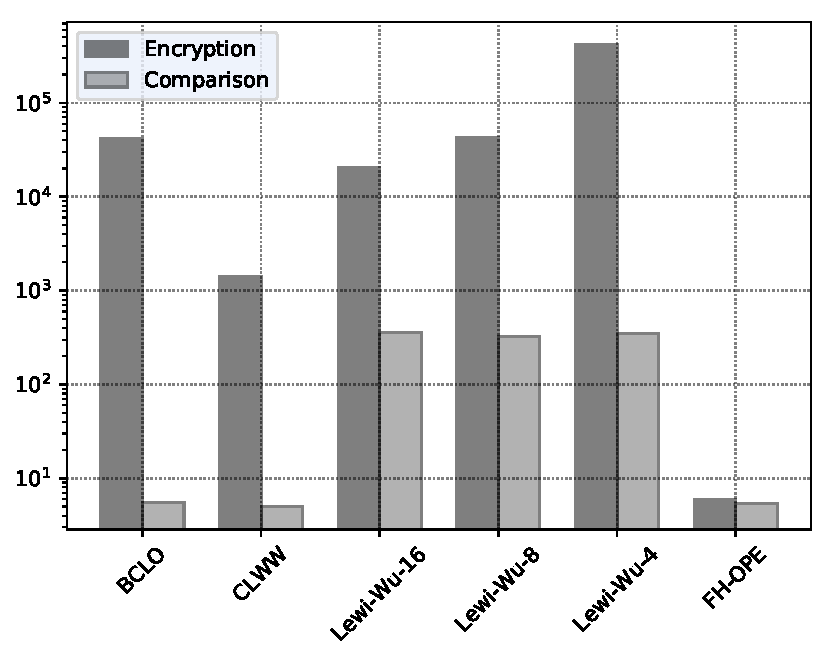
\includegraphics[width=\linewidth]{schemes-benchmark}
% 		\caption{Schemes benchmark (time in microseconds, log scale). Lewi-Wu parameter is the number of blocks.}
% 	\end{subfigure}%
% 	~ % chktex 39
% 	\begin{subfigure}[t]{0.5\linewidth}
% 		\centering
% 		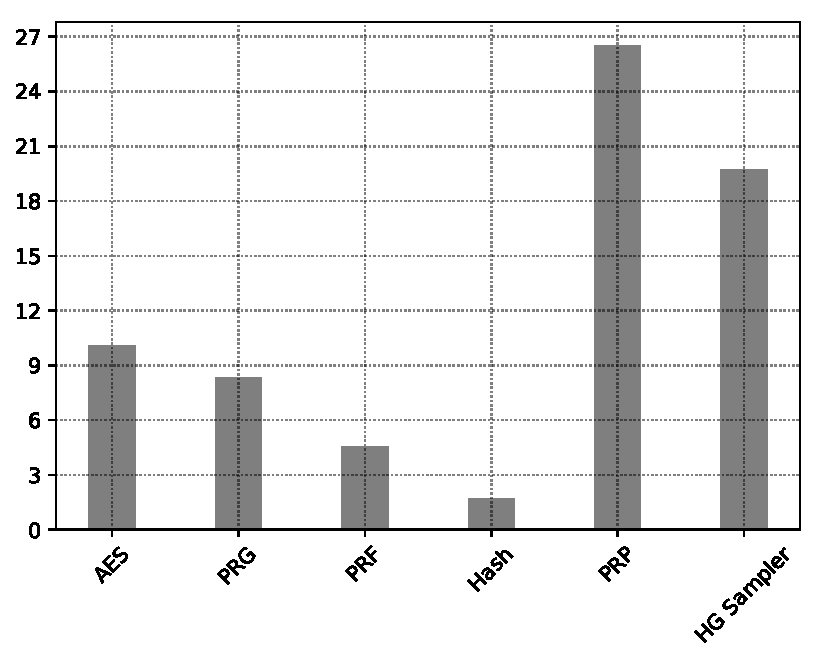
\includegraphics[width=\linewidth]{primitives-benchmark}
% 		\caption{Primitives benchmark (time in microseconds)}
% 	\end{subfigure}%
% 	\caption{Benchmarks of the schemes and primitives}\label{figure:benchmarks}
% \end{figure}

\begin{figure}[!ht]
	\centering
	\begin{minipage}[t]{0.48\columnwidth}
		\centering
		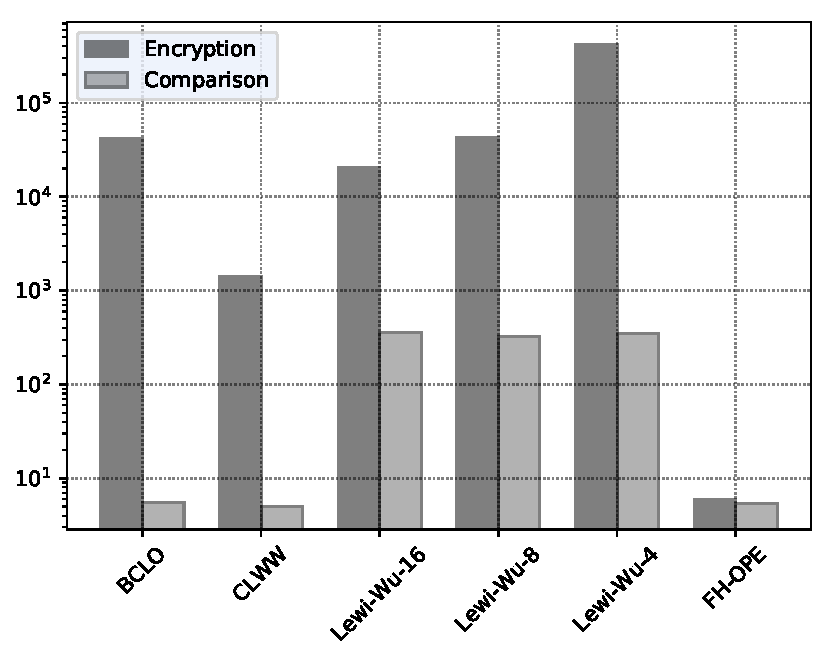
\includegraphics[width=\linewidth]{schemes-benchmark}
		\captionof{figure}{Schemes benchmark (time in microseconds, log scale). Lewi-Wu parameter is the number of blocks.}%
		\label{figure:benchmarks:schemes}
	\end{minipage}
	~ % chktex 39
	\begin{minipage}[t]{0.48\columnwidth}
		\centering
		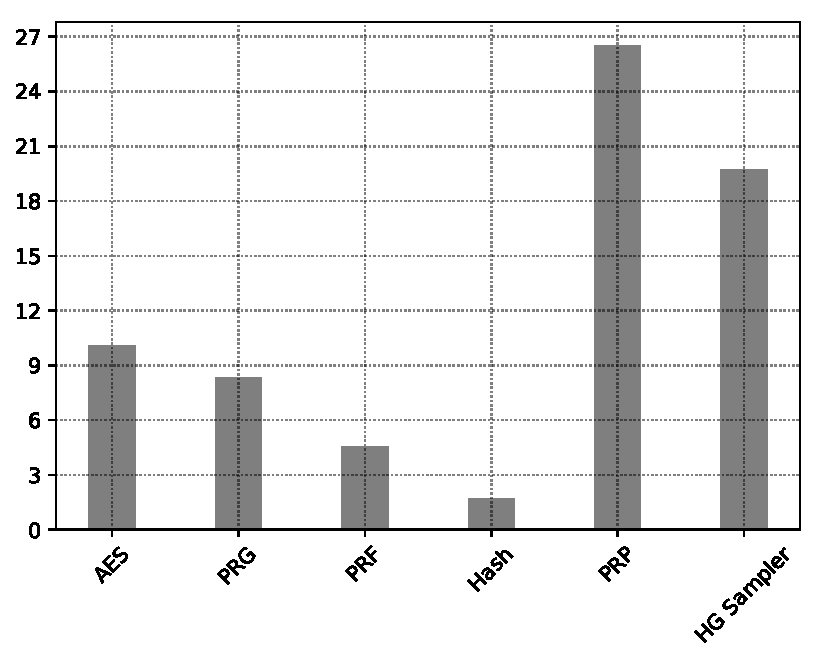
\includegraphics[width=\linewidth]{primitives-benchmark}
		\captionof{figure}{Primitives benchmark (time in microseconds)}%
		\label{figure:benchmarks:primitives}
	\end{minipage}
\end{figure}


		\subsubsection{Simulations}

			\begin{figure*}[ht!]
	\captionsetup[subfigure]{justification=centering}
	\centering
	\begin{subfigure}[t]{0.5\textwidth}
		\centering
		
\includegraphics[width=\linewidth]{protocol-charts-cios}
		\caption{Construction stage number of \acrshort{io} requests}%
		\label{figure:protocols-ios:c}
	\end{subfigure}%
	\hfill
	\begin{subfigure}[t]{0.5\textwidth}
		\centering
		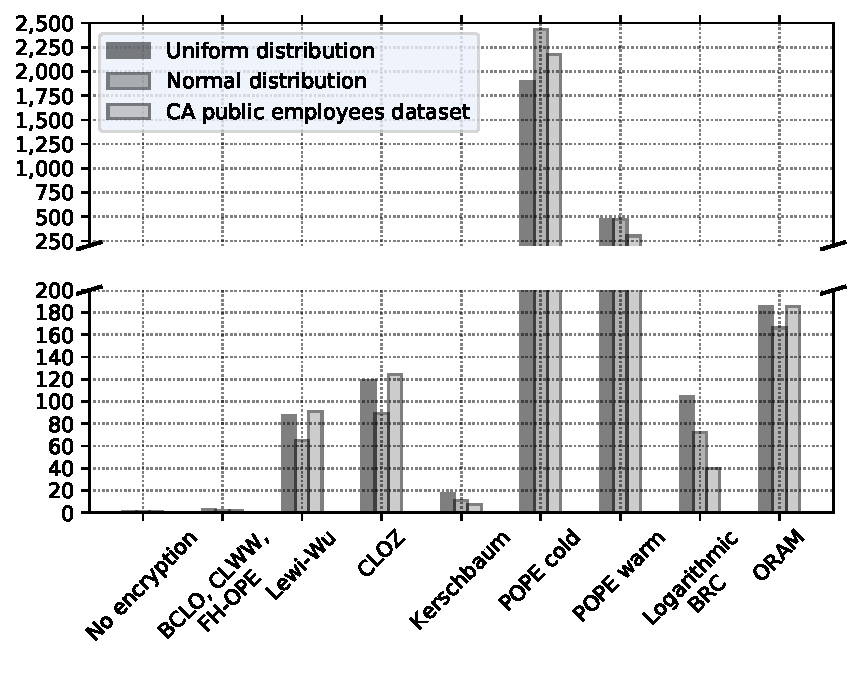
\includegraphics[width=\linewidth]{protocol-charts-qios}
		\caption{Queries stage number of \acrshort{io} requests}%
		\label{figure:protocols-ios:q}
	\end{subfigure}%
	\caption{Number of \acrshort{io} requests for different protocols and data distributions}%
	\label{figure:protocols-ios}
\end{figure*}

\begin{figure*}[ht!]
	\captionsetup[subfigure]{justification=centering}
	\centering
	\begin{subfigure}[t]{0.5\textwidth}
		\centering
		
\includegraphics[width=\linewidth]{protocol-charts-csize}
		\caption{Construction stage communication size (bytes transferred)}%
		\label{figure:protocols-size:c}
	\end{subfigure}%
	\hfill
	\begin{subfigure}[t]{0.5\textwidth}
		\centering
		
\includegraphics[width=\linewidth]{protocol-charts-qsize}
		\caption{Queries stage communication size (transferred bytes, log scale)}%
		\label{figure:protocols-size:q}
	\end{subfigure}%
	\caption{Communication size for different protocols and data distributions}%
	\label{figure:protocols-size}
\end{figure*}

\begin{figure*}[ht!]
	\captionsetup[subfigure]{justification=centering}
	\centering
	\begin{subfigure}[t]{0.5\textwidth}
		\centering
		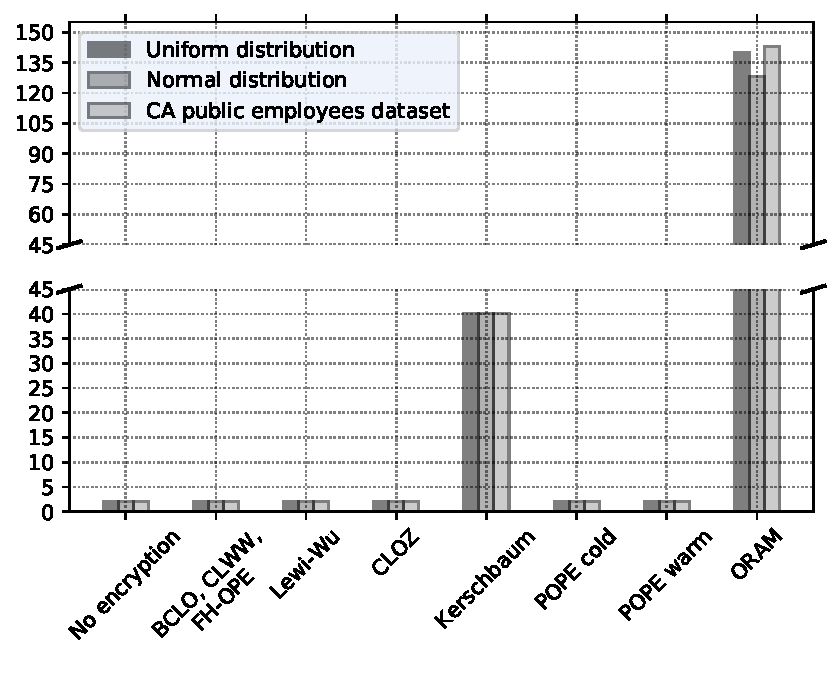
\includegraphics[width=\linewidth]{protocol-charts-cvol}
		\caption{Construction stage communication volume (number of messages)}%
		\label{figure:protocols-vol:c}
	\end{subfigure}%
	\hfill
	\begin{subfigure}[t]{0.5\textwidth}
		\centering
		
\includegraphics[width=\linewidth]{protocol-charts-qvol}
		\caption{Queries stage communication volume (number of messages)}%
		\label{figure:protocols-vol:q}
	\end{subfigure}%
	\caption{Communication volume for different protocols and data distributions}%
	\label{figure:protocols-vol}
\end{figure*}


			We have four types of simulations.

			Protocol simulation runs both protocol stages --- construction and search --- on supplied data for all protocols including all schemes coupled with {\BPlus} tree.
			In this simulation we measure the primitive usage, number of \acrshort{ore} scheme operations (when applies), communication volume and size, and the number of \acrshort{io} requests.
			We intentionally do not measure elapsed time, since it would be extremely inaccurate in this setting --- simulation and measurement routines take substantial fraction of time.

			Scheme simulation runs all five \acrshort{ore} schemes and tracks only the primitive usage.

			The scheme benchmark, however, is designed to track time.
			We use Benchmark.NET \cite{benchmark-net} to ensure that the reported time is accurate.
			This tool handles issues like cold / warm start, elevating process' priority, and performing enough runs to draw statistically sound conclusions.
			This benchmark reports elapsed time up to nanoseconds for all four schemes (excluding CLOZ \cite{parameter-hiding-ore}) and their variants.

			Finally, primitive benchmark uses the same tool, but compares the primitives.
			We use it to compare different implementations of primitives (e.g.\ Feistel \acrshort{prp} vs pre-generated permutation) and to approximate time consumption of the schemes and protocols based on primitive usage.

	\subsection{Setup}

		For our simulations, we have used three datasets.
		Two synthetic distributions, that are uniform (range is third of data size) and normal (standard deviation is $0.1$ of data size).
		The real dataset is California public employees salaries (``total pay and benefits'' column) \cite{ca-dataset}.
		Synthetic datasets and subsets of the real dataset are generated pseudo\hyp{}randomly.
		Queries are generated uniformly at random with a range as a percentage of data size.

	\subsection{Results}

		\subsubsection{Primitive usage by schemes}\label{section:range-snapshot:schemes-primitive-usage}

			In \cref{table:primitive-usage-theory} we show the simulation-derived values of each \acrshort{ope} and \acrshort{ore} scheme's primitive usage.
			Each scheme is given \num{1000} data points of each dataset.
			First, the scheme encrypts each data point, then decrypts each ciphertext and then performs five comparisons (all possible types) pairwise.
			This micro-simulation is repeated \num{100} times.
			Resulting values for primitive usage are averaged for each scheme.
			State and ciphertext sizes are calculated after each operation and the values are averaged.
			Please note that the simulated values are consistent with the theoretical calculations.

		\subsubsection{Benchmarks of schemes and primitives}

			Using the Benchmark.NET tool \cite{benchmark-net}, we have accurately tracked the performance of the schemes and primitives running of different parameters (see \cref{figure:benchmarks:schemes,figure:benchmarks:primitives}).
			\acrshort{ore} schemes benchmark setup is the same as in primitive usage simulation \cref{section:range-snapshot:schemes-primitive-usage}.
			Primitives were given randomly generated byte inputs and keys of different sizes (e.g.\ \acrshort{prp} of $2$ to $32$ bits).
			Benchmark.NET decides how many times to run the routine to get statistically sound results.
			For example, large variance results in more runs.
			To improve the accuracy, each run is compiled in release mode as a separate project and runs in a separate process with the highest priority.

			Please note the logarithmic scale of the schemes' performances.
			FH-OPE is fast since it does not perform \acrshort{cpu}-heavy operations and works in main memory.
			Lewi-Wu performance degrades exponentially with the increase of block size mainly due to exponential number of \acrshort{prf} executions and the performance of \acrshort{prp} degrading exponentially.
			Note also that Lewi-Wu comparison takes noticeable time due to Hash primitive usage.

			In the primitives benchmark, it is clear that most primitives use \acrshort{aes} under the hood.
			\acrshort{prg} and \acrshort{prf} take less than \acrshort{aes} because they do not include the initialization vector generation needed for symmetric encryption.
			\acrshort{prp} is implemented as a Knuth shuffle \cite{knuth-shuffle} and its complexity is exponential in the input bit length.
			Input size of 2 bits is shown on \cref{figure:benchmarks:schemes}.
			\acrshort{prg} does not discard the entropy generated by \acrshort{aes} cycle, so one \acrshort{aes} cycle can supply four 32-bit integers.
			\acrshort{prp} generates the permutation table once and does not regenerate it if the same key and number of bits are supplied.

		\subsubsection{Protocols}\label{section:range-snapshot:results-protocols}

			In this experiment we have run each protocol with each of the three datasets.
			Dataset sizes are \num{247000} (bounded by California Employees dataset size) and the number of queries is \num{1000}.
			Queries are generated uniformly at random with a fixed range --- \SI{0.5}{\percent} of data size.
			The cache size is fixed to \num{128} blocks, and the {\BPlus} tree branching factor as well as block sizes for other protocols are set such that the page size is \SI{4}{\kibi\byte}.
			The values we are measuring are the number of \acrshort{io} operations, communication volume, and size for both construction and query stages.

			See \cref{table:protocols} for the snapshot for particular distribution (CA employees).
			\cref{figure:protocols} shows all values we tracked for all protocols and distributions.
			Values for \acrshort{ore} based protocols are averaged.
			Being ``cold'' in our simulations means executing the first query and being ``warm'' means the first query has been previously executed.
			This difference makes sense only for POPE as its first query incurs disproportionately large overhead by design.

			Note that all \acrshort{ore} based protocols behave the same except when ciphertext size matters.
			Thus, since BCLO, CLWW and FH-OPE have the same ciphertext size, they create {\BPlus} trees with the same page capacity and have the same number of \acrshort{io}s for different operations.
			Lewi-Wu and CLOZ schemes have relatively large ciphertexts and thus induce larger traffic (see \cref{figure:protocols:csize}) and smaller {\BPlus} tree branching factor resulting in greater number of \acrshort{io} requests (see \cref{figure:protocols:qios}).
			Kerschbaum protocol requires high number of \acrshort{io} requests during construction since it needs to insert an element into the arbitrary place in an array and rotate the data structure on a disk.

			POPE suffers huge penalty on the first query (see \cref{figure:protocols:qios,figure:protocols:qvol,figure:protocols:qsize}) since it reads and sends all blocks to the client for sorting.
			POPE performance improves as more queries are executed.

			Logarithmic-BRC does not support interactive insertions and thus its construction stage is not benchmarked.
			Otherwise it is the most performant of all non-\acrshort{ore} protocols.
			Note, however, that its performance depends on the result size, not data size.

			As expected, \acrshort{oram} performs worse than the \acrshort{ore}-based protocols, but its performance is in-line with the non-\acrshort{ore} protocols.
			It may seem that \acrshort{oram} does especially bad in construction communication (\cref{figure:protocols:qvol,figure:protocols:qsize}), but it is only because POPE has a shortcut in construction.
			This ``debt'' is being payed off during queries (\cref{figure:protocols:qsize}).

			Note that the values do not vary a lot among different data distributions except for \acrshort{io} requests.
			\acrshort{io} performance depends on the result size for queries, and is therefore more sensitive to data distribution.

			Also note that using an \acrshort{ore} scheme with relatively small ciphertext in {\BPlus} tree does not add any substantial \acrshort{io} overhead (see ``No encryption'').

			On \cref{figure:protocols-query-sizes} it is clear that query performance does not depend substantially on the query size, except for Logarithmic-BRC, for which the relation is linear.
			Note that Logarithmic-BRC with optimally configured \texttt{pack} extension shows almost no growth.
			This is because for large ranges \acrshort{brc} will return the higher nodes (keywords matching many documents), which are optimally packed in \acrshort{io} pages.
			As query range doubles, higher nodes are involved increasing the chance that requested keywords have their documents packed.

			\newlength{\hardcodedheighto}
\newlength{\askipo}
\newlength{\bskipo}
\newlength{\blskipo}

\setlength{\hardcodedheighto}{135pt}
\setlength{\askipo}{-10pt}
\setlength{\bskipo}{0pt}
\setlength{\blskipo}{-5pt}

\begin{figure*}[ht!]	
	\captionsetup{justification=centering}
	\centering
	\begin{minipage}{0.66\textwidth}
		\captionsetup[subfigure]{justification=centering}
		\centering
		\begin{subfigure}[t]{0.5\textwidth}
			\centering
			
\includegraphics[height=\hardcodedheighto,width=\linewidth]{protocol-data-percent-cios.pdf}
			\setlength{\abovecaptionskip}{\askipo}
			\setlength{\belowcaptionskip}{\bskipo}
			\caption{Construction stage {\IO} requests}\label{fig:protocols-data-percent:cios}
		\end{subfigure}%
		~ % chktex 39
		\begin{subfigure}[t]{0.5\textwidth}
			\centering
			
\includegraphics[height=\hardcodedheighto,width=\linewidth]{protocol-data-percent-cvol.pdf}
			\setlength{\abovecaptionskip}{\askipo}
			\setlength{\belowcaptionskip}{\bskipo}
			\caption{Construction stage number of messages}\label{fig:protocols-data-percent:cvol}
		\end{subfigure}%
	
		\begin{subfigure}[t]{0.5\textwidth}
			\centering
			
\includegraphics[height=\hardcodedheighto,width=\linewidth]{protocol-data-percent-qios.pdf}
			\setlength{\abovecaptionskip}{\askipo}
			\setlength{\belowcaptionskip}{\blskipo}
			\caption{Queries stage {\IO} requests}\label{fig:protocols-data-percent:qios}
		\end{subfigure}%
		~ % chktex 39
		\begin{subfigure}[t]{0.5\textwidth}
			\centering
			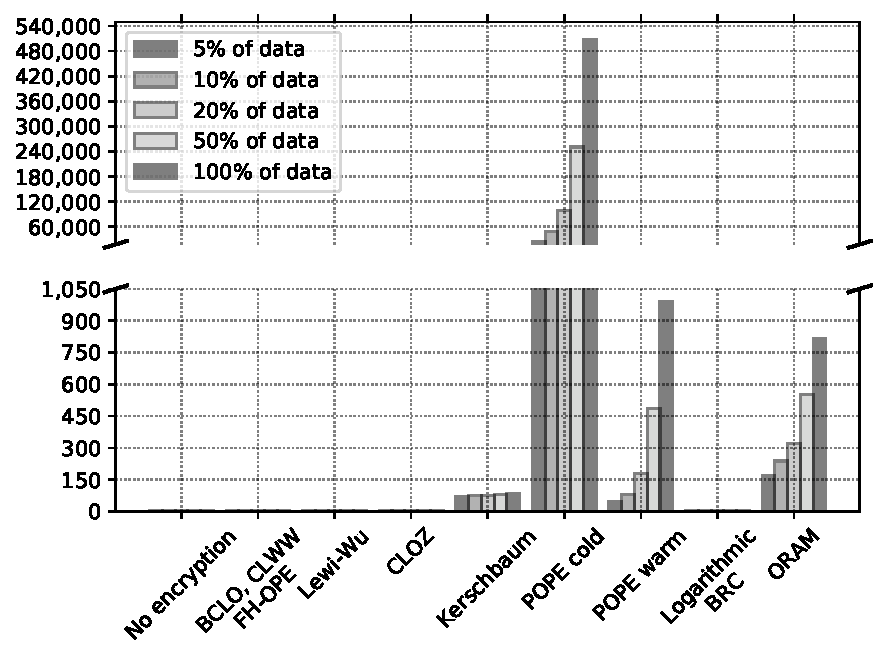
\includegraphics[height=\hardcodedheighto,width=\linewidth]{protocol-data-percent-qvol.pdf}
			\setlength{\abovecaptionskip}{\askipo}
			\setlength{\belowcaptionskip}{\blskipo}
			\caption{Queries stage number of messages}\label{fig:protocols-data-percent:qvol}
		\end{subfigure}%
		\caption{Protocol scalability}\label{fig:protocols-data-percent}
	\end{minipage}%
	\begin{minipage}{.33\textwidth}
		\captionsetup[subfigure]{justification=centering}
		\centering
		\begin{subfigure}[t]{\textwidth}
			\centering
			\setlength{\abovecaptionskip}{-0pt}
			\setlength{\belowcaptionskip}{\bskipo}
			
\includegraphics[height=\hardcodedheighto,width=\linewidth]{protocol-query-sizes-ios.pdf}
			\caption{For different query sizes}\label{fig:protocols-query-sizes}
		\end{subfigure}%

		\begin{subfigure}[t]{\textwidth}
			\centering
			
\includegraphics[height=\hardcodedheighto,width=\linewidth]{cold-vs-warm-ios.pdf}
			\setlength{\abovecaptionskip}{\askipo}
			\setlength{\belowcaptionskip}{\blskipo}
			\caption{Over time (queries).}\label{fig:cold-vs-warm}
		\end{subfigure}%
		\caption{Number of {\IO} requests}\label{fig:protocols-different-queries}
	\end{minipage}
\end{figure*}


			\cref{figure:protocols-data-percent} shows \cref{table:protocols} asymptotic values.
			The simulation was run for uniform dataset of \num{247000} records (hundred percent), \num{1000} queries, \SI{0.5}{\percent} query range and \num{128} blocks cache size.
			Kerschbaum construction \acrshort{io}s and cold POPE query values grow linearly with inputs, while the other protocols grow logarithmically, square-logarithmically, or do not grow.

			\cref{figure:cold-vs-warm} shows how the performance of protocols fluctuates as queries are processed.
			Note that POPE and Logarithmic-BRC fluctuate the most (which is, in general, undesirable), and POPE is the only protocol where cold versus warm makes a difference.

